\section{Businessplan}
\subsection{Gründerpersonen}
	\begin{description}
	\item [Vorstellung und Qualifikationen] \hfill \\
		Das Gründungsteam besteht aus Addis Dittebrandt, Kai Frank Roßwag, Peter Noras und Yannick Tanner.
			Wir sind vier Bachelor Informatik Studenten am KIT in Karlsruhe. Im Rahmen des Proseminars Sensorgetriebene Information Appliances haben wir uns Kenntnisse in der Programmierung von sensorgesteuerten Applikationen angeeignet. Zusätzlich zur Realisierung des DryR haben wir aufgrund des Nebenfachs BWL grundlegende kaufmännische Fähigkeiten in die Realisierung des Projekts einbringen können.
	\end{description}
\subsection{Unser Produkt}
	Wir haben während des Proseminars den DryR entwickelt. Der DryR dient der Überwachung des Trocknungsvorgangs von auf der Wäscheleine hängender Kleidung. \\

	Die Besonderheit an unserer Geschäftsidee ist, dass wir ein Monopol besitzen. Bisher gibt es keine intelligente Wäscheklammer, die Ihnen auf dem Smartphone anzeigt ob ihre Wäsche trocken ist. Wir haben bereits einen Prototyp gebaut und die App ist auf Android-Smartphones über eine APK installier- und ausführbar. Wir streben an 100 Premium DryR im ersten Jahr zu verkaufen und somit unsere Entwicklungskosten zu decken. Ein Patent ist angestrebt, jedoch aus Mangel finanzieller Mittel nicht in die Wege geleitet. Erste Test wurden bereits erfolgreich abgeschlossen. Langfristig streben wir an, dass in jedem Trocknungsraum im Keller oder Dachboden der DryR nicht mehr weg zu denken ist. Wir bieten hierbei zwei Modelle:

	Das Basismodell - Beinhaltet eine Wäscheklammer und die App.

	Das Premiummodell - Beinhaltet zusätzlich die Basisstation sowie erweiterte Funktionalität.

	Zudem lässt sich durch eine geringe Modifikation der DryR zu einem Feuchtigkeitssensor umprogrammieren, wodurch in Lagerhallen die Feuchte der Kleidung gemessen werden kann um Schaden durch z. B. Schimmel vorzubeugen.

\subsection{User Story}
	Johannes ist Maschinenbaustudent im 2. Semester an der Technischen Universität Neustadt. Er lebt mit zwei weiteren Studenten in einer WG im dritten Stock. Die Studenten teilen sich neben Küche und einem Gemeinschaftsraum auch ein kleines Kellerabteil, neben dem auch eine gemeinschaftlich genutzte Waschmaschine steht. Üblicherweise kommt Johannes mit seinen Mitbewohnern gut aus, aber manchmal kommt es zu Problemen, wenn etwa morgens alle ins Bad müssen oder Dinge nicht rechtzeitig weggeräumt werden. Insbesondere sein Mitbewohner Markus ärgert sich oft über Johannes, etwa wenn seine Klamotten viel zu lange an der zu eng bemessenen Wäscheleine im Keller hängen. Allerdings hat Johannes auch nicht immer die Zeit oder die Lust dazu, seine Studien zu unterbrechen und die vier Treppen in den Keller herunterzulaufen, nur um festzustellen, dass sein dicker Pullover immer noch nicht ganz trocken ist und er noch einmal laufen muss.

\subsection{Markt und Wettbewerb}
	Ein solches Produkt existiert noch nicht, jedoch gibt es viele Haushalte mit Trocknern, die in diesem Fall als Interessenten weg fallen. \\

	Unsere Kunden setzen sich aus jungen Erwachsenen zusammen, die ihre Wäsche im Keller oder Dachboden trocknen. Da Platz in solchen Trocknungsräumen meist Mangelware ist und die Wäsche nicht unnötig in diesen Räumen hängen muss. Die Kunden sind zwischen 18 und 45 Jahre alt. Bei einer Umfrage von 250 Personen haben wir bereits 40 potenzielle Kunden für unser Basisprojekt begeistern können.

\subsection{Marketing}
		Bisher haben wir noch keine Werbung geschalten und uns nur über direkten Kundenkontakt Interessenten gesichert

			Durch den Vertrieb über das Internet und Plattformen wie Amazon oder eBay bleiben die Kosten für den Vertrieb überschaubar. Eine Angliederung an eine Teleshoppingkanal ist ebenfalls nicht auszuschließen. Da wir noch in der Entwicklungsphase stecken und noch keine Angebote von Sensor- und Platinenherstellern einholen konnten, rechnen wir mit den Kosten für den Prototypen. Der Preis setzt sich wie folgt zusammen:
\begin{table}[htbp]
  \centering
  \caption{Verkaufspreis}
    \begin{tabularx}{\textwidth}{|X|XX|}
    \toprule
    & Kosten & Verkaufspreis\\
    \midrule
    Sensor & 4,00 € & 6,00 € \\
    Basisstation & 35,00 € & 55,00 € \\
    Entwicklung & 6.000,00 € & - \\
    \bottomrule
    \end{tabularx}%
  \label{tab:addlabel}%
\end{table}%

\begin{table}[htbp]
	\centering
	\caption{Kostendeckungspunkt}
	\begin{tabularx}{\textwidth}{|X|XX|}
		\toprule
		& Verkaufspreis & Gewinn nach Einzelverkäufen \\
		\midrule
		Verkauf Basis & 10,00 € & 603,9 \\
		 Verkauf Premium & 60,00 € & 100,65 \\
		\bottomrule
	\end{tabularx}%
	\label{tab:addlabel}%
\end{table}%

\subsection{Mitarbeiter}
	Da wir bisher noch in der Entwicklungsphase sind, sind nur die Gründer als Mitarbeiter beschäftigt. 
			
\subsection{Risiken/Chancen}
	Wir sehen eine Chance uns mit unserem Monopol auf dem Markt behaupten zu können. 
	Sobald wir die Entwicklung abgeschlossen haben und ein Patent erteilt wurde, würden wir mit ihrem Investment Werbung schalten und unser Produkt weltweit bekannt machen. Als Risiko sehen wir, dass viele Familien einen Trockner besitzen und somit das Aufhängen der Wäsche entfällt. Jedoch ist unser Produkt umweltbewusster.

\addtocounter{subsection}{1}
\addcontentsline{toc}{subsection}{\protect\numberline{\thesubsection}Finanzplan}
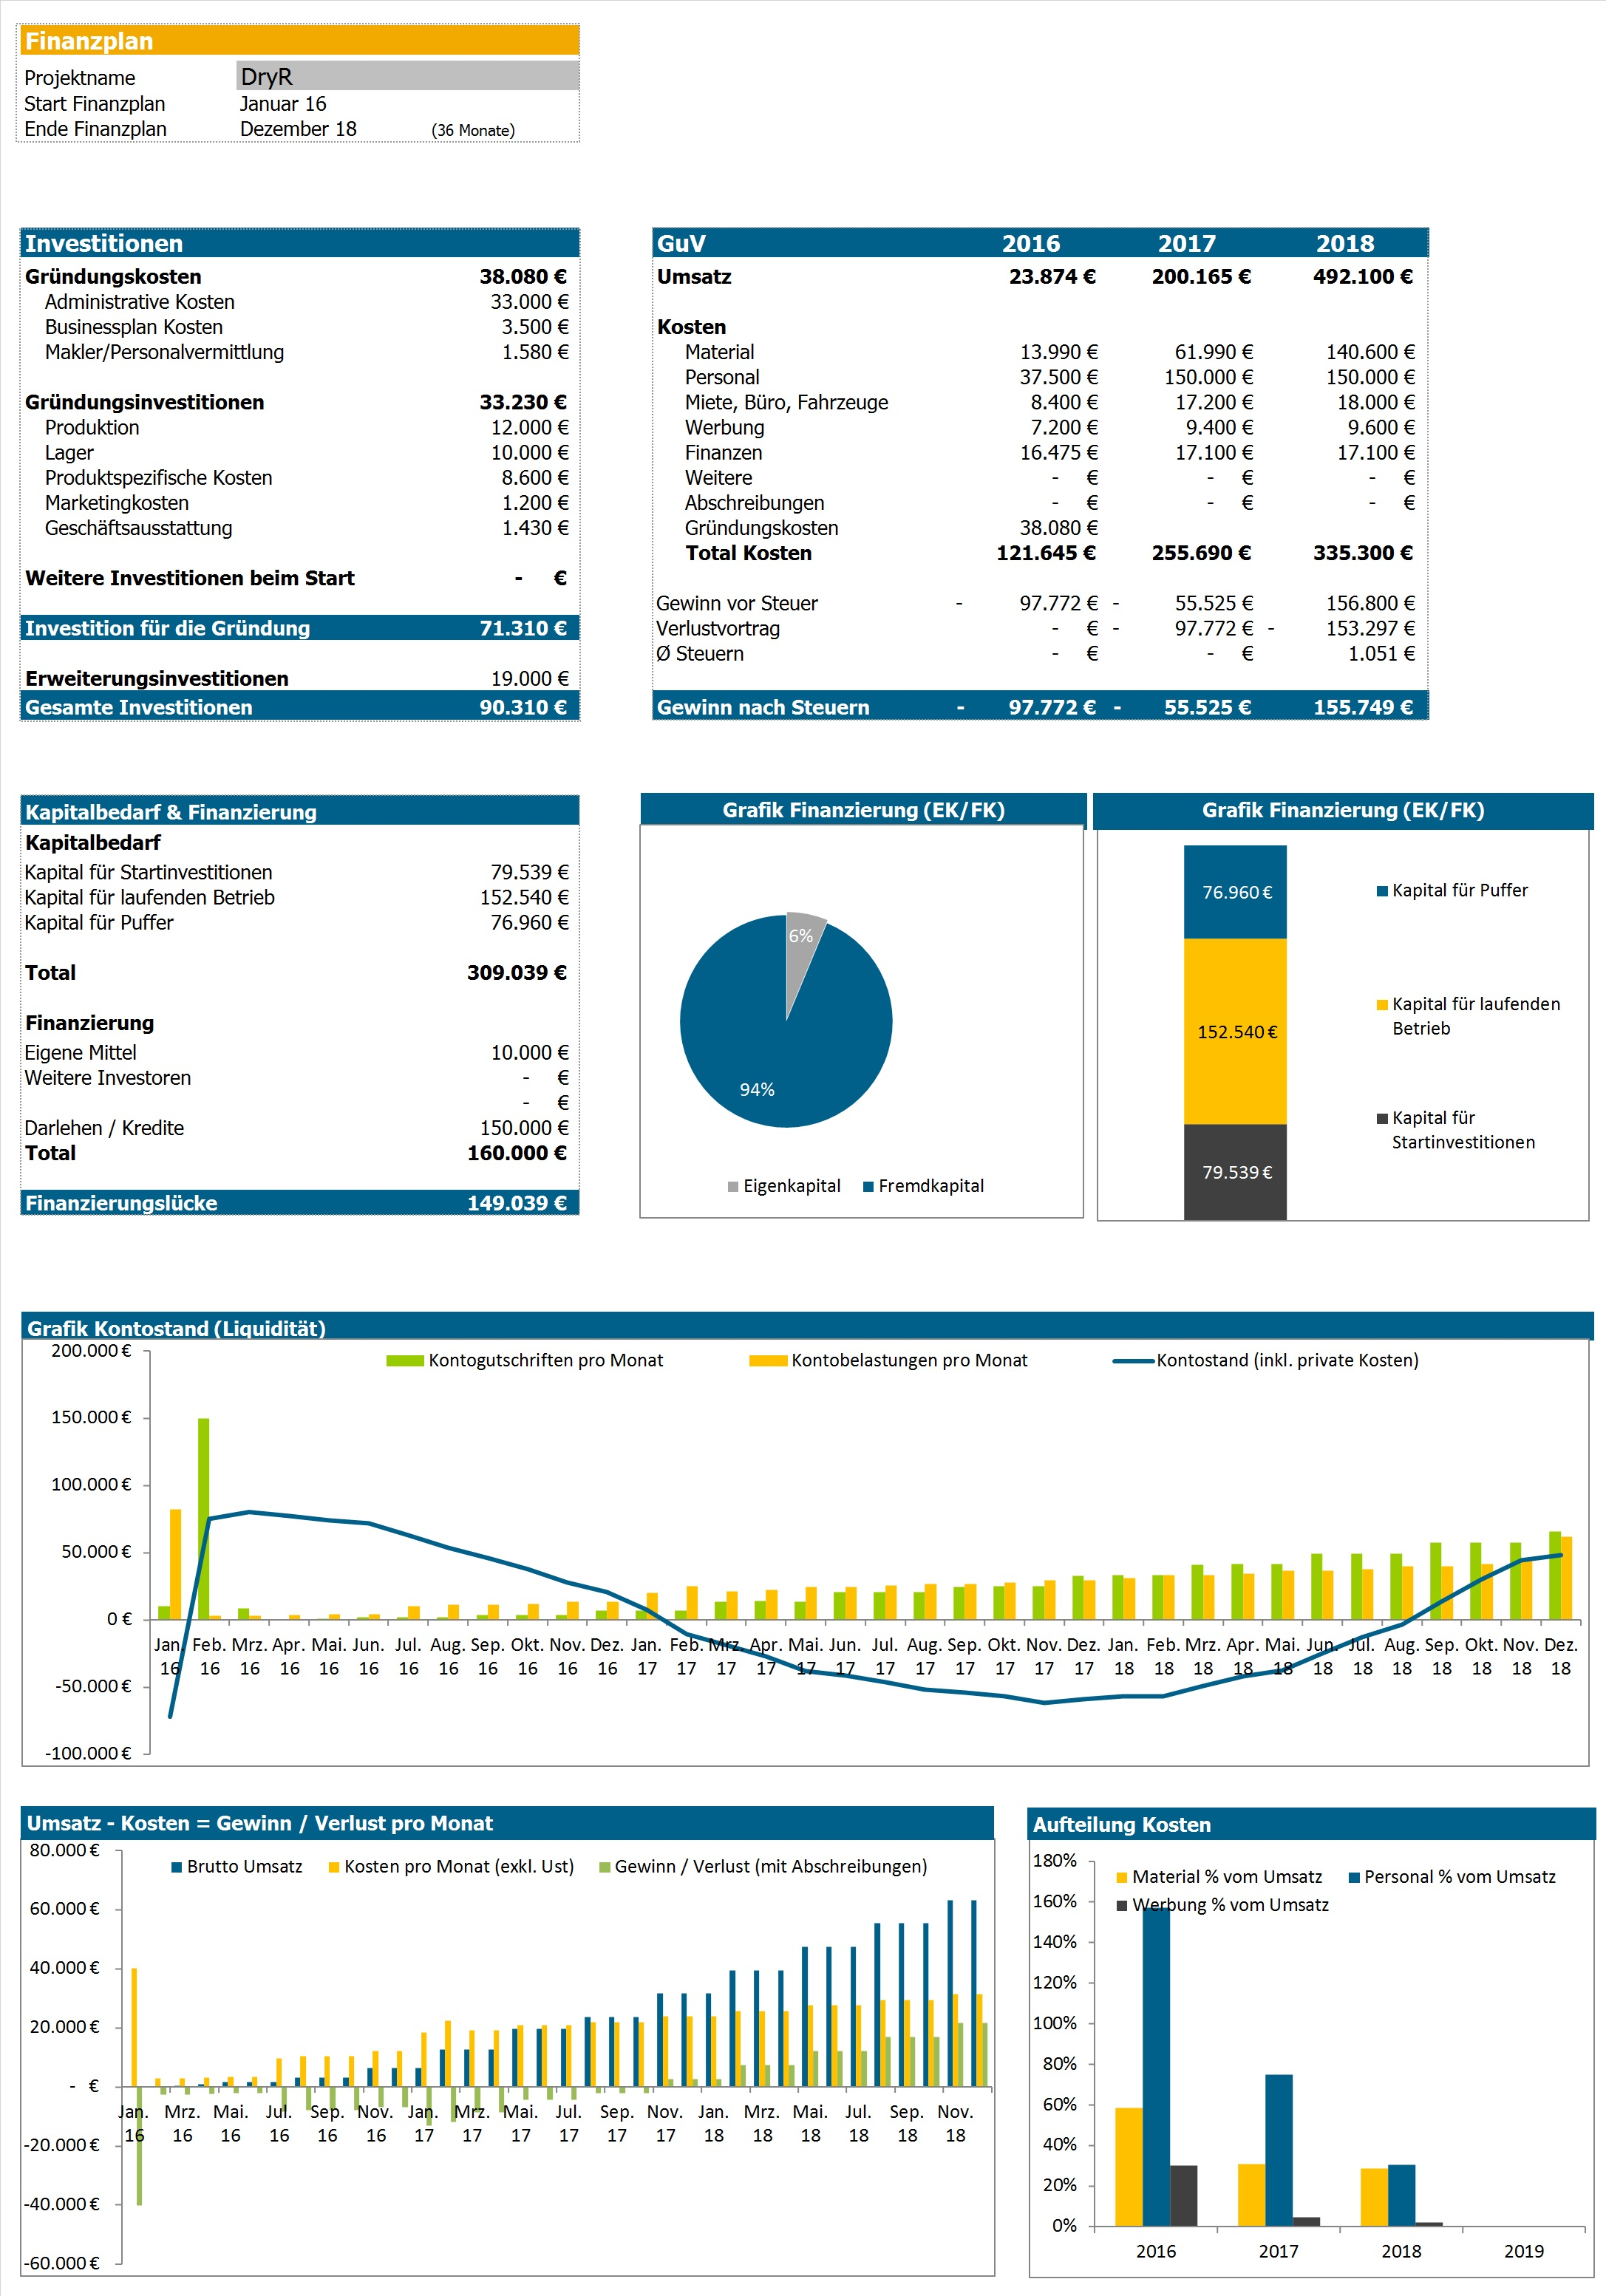
\includepdf{Finanzplan.jpg}
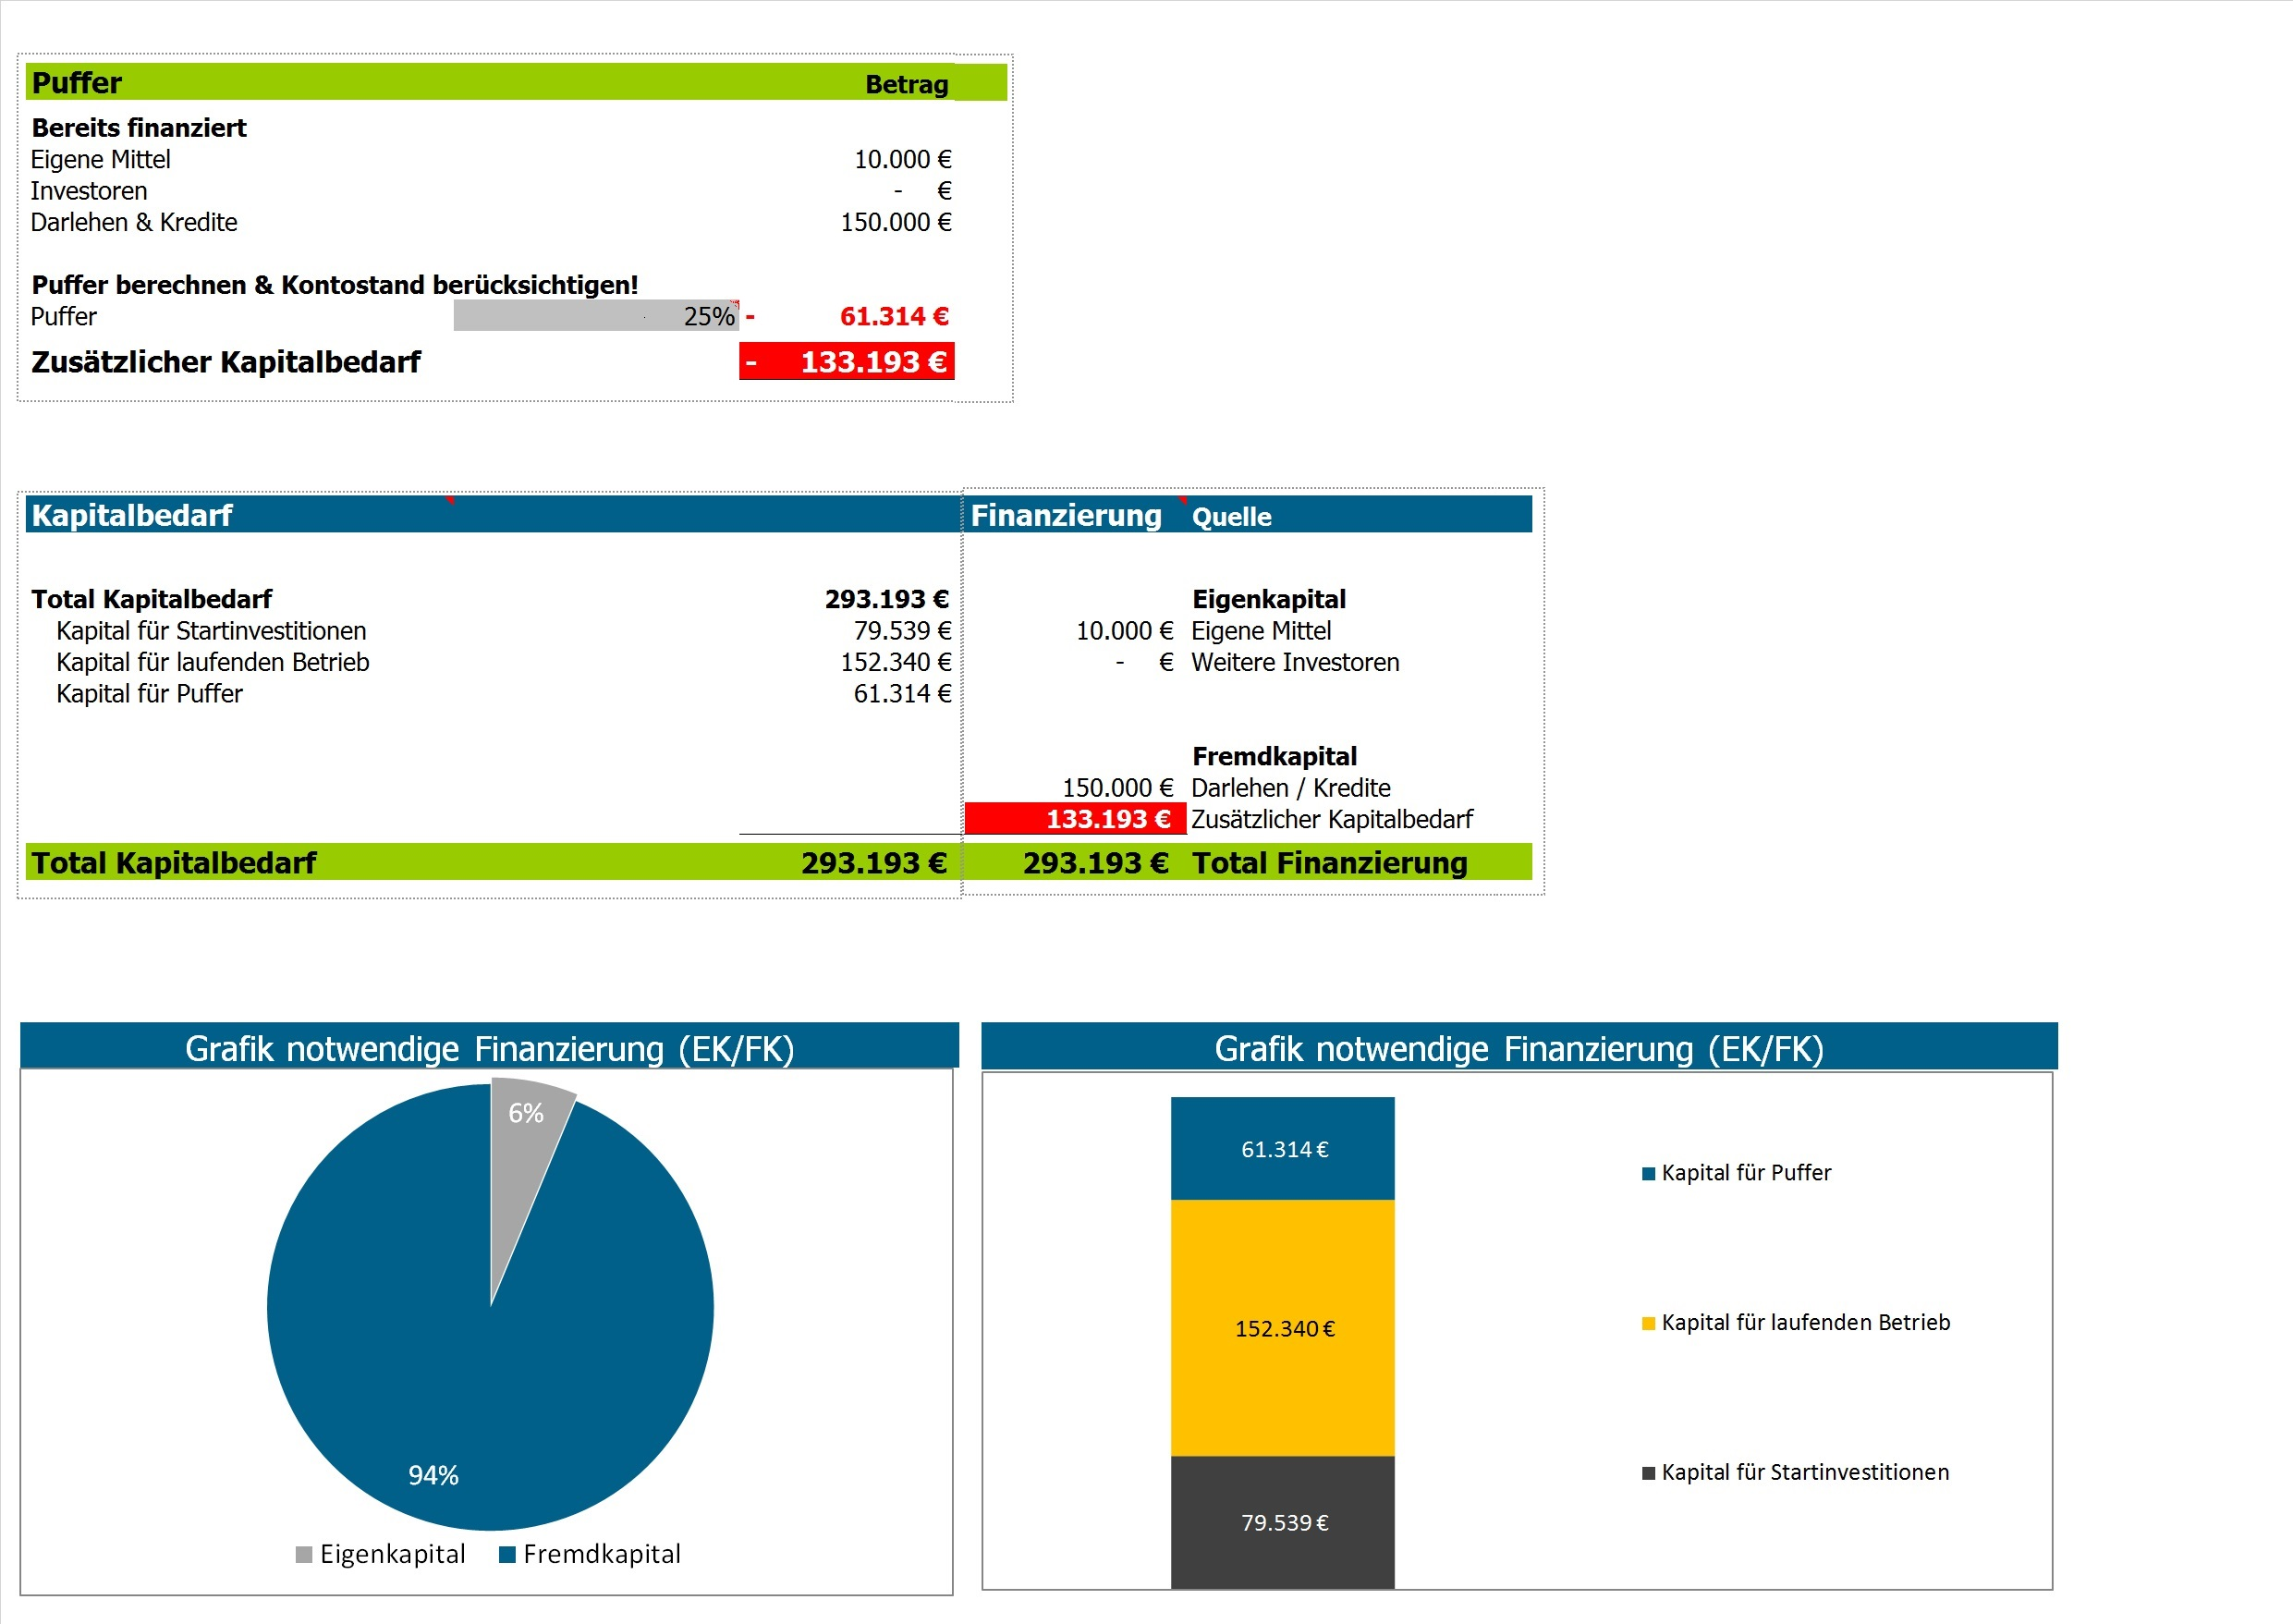
\includepdf{Kapitalbedarf.jpg}
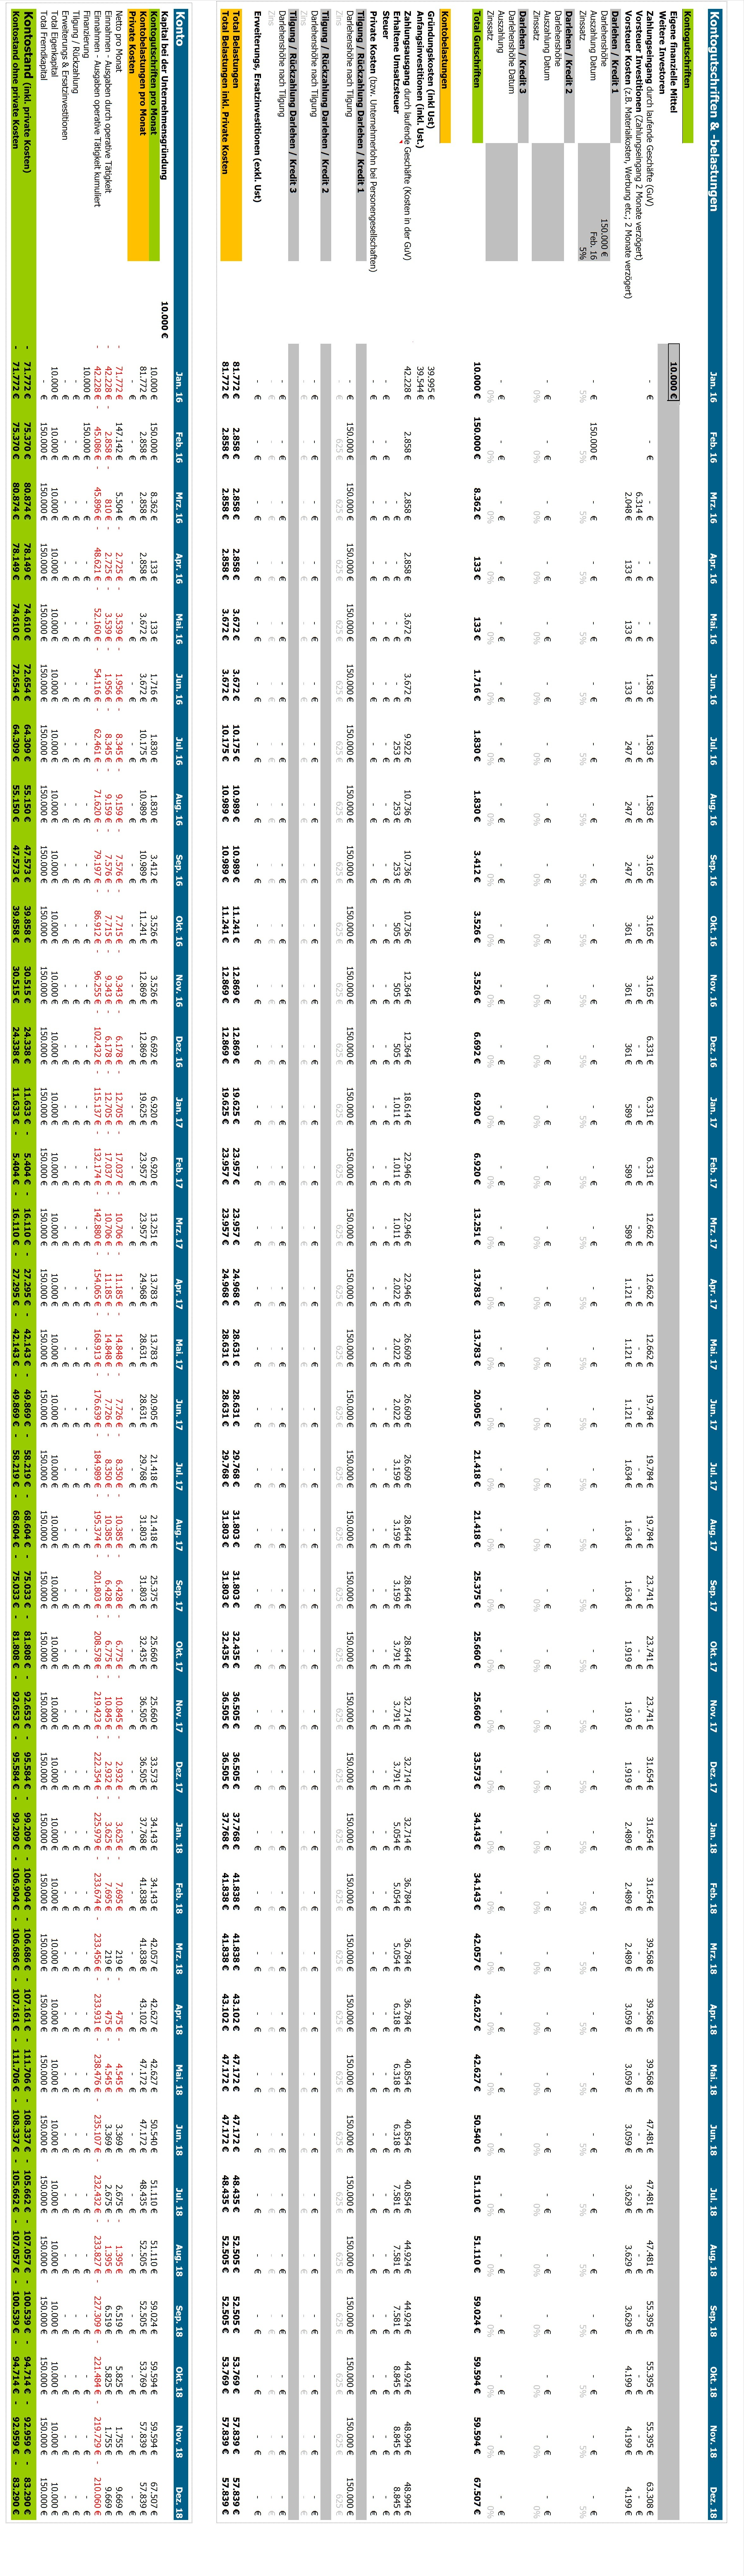
\includepdf{Liqiditaet_rotated.jpg}
